\clearpage
\section{Analiza technologii i architektura systemu}		%3

W rozdziale przedstawiono najważniejsze technologie wykorzystane w projekcie oraz ogólną architekturę aplikacji. System został zaprojektowany jako aplikacja desktopowa, ponieważ taki sposób działania pozwala operatorowi uruchomić monitoring lokalnie, bez konieczności wdrażania serwera WWW lub dodatkowej infrastruktury sieciowej.

\subsection{Zastosowane technologie i biblioteki}

Do budowy systemu wykorzystano język Python oraz zestaw bibliotek przeznaczonych do przetwarzania obrazu, uczenia maszynowego i tworzenia interfejsów graficznych. Dobór bibliotek oparto na ich zastosowaniu w zadaniach detekcji obiektów, przetwarzania obrazu i budowy aplikacji desktopowych. Ważne było również to, aby użyte narzędzia pozwalały uruchomić aplikację lokalnie, obsłużyć wiele źródeł obrazu i wygodnie zmieniać parametry modeli bez przebudowy całego projektu.

\begin{itemize}
\item \textbf{Python} -- główny język implementacji aplikacji, skryptów treningowych oraz narzędzi pomocniczych \cite{pythondocs}.
\item \textbf{Ultralytics YOLO} -- biblioteka używana do detekcji osób, segmentacji sylwetek oraz obsługi wariantów modeli YOLO. Rodzina YOLO została zaprojektowana z myślą o detekcji w czasie rzeczywistym \cite{redmon2016yolo}, a implementacja Ultralytics udostępnia między innymi zadania detekcji, segmentacji i trackingu \cite{ultralyticsdocs}.
\item \textbf{PyTorch} -- środowisko uruchomieniowe dla modeli głębokiego uczenia, z możliwością pracy na GPU \cite{paszke2019pytorch,pytorchdocs}.
\item \textbf{OpenCV} -- biblioteka odpowiedzialna za odczyt obrazu z kamer, plików wideo i strumieni, a także za zapis klipów zdarzeń \cite{opencvdocs}.
\item \textbf{PyQt6} -- biblioteka użyta do stworzenia graficznego interfejsu operatora \cite{pyqtdocs}.
\item \textbf{YAML} -- format plików konfiguracyjnych, wykorzystywany do przechowywania ustawień inferencji, treningu i datasetu \cite{yamlspec}.
\end{itemize}

Dobór technologii wynikał z potrzeby połączenia kilku obszarów: detekcji obiektów w czasie zbliżonym do rzeczywistego, wygodnego interfejsu użytkownika oraz możliwości późniejszego treningu i wymiany modeli.

\subsection{Zakres wykorzystania narzędzi}

Python pełni rolę języka łączącego wszystkie części systemu. W aplikacji odpowiada za logikę interfejsu, obsługę konfiguracji, sterowanie wątkami odczytu obrazu, komunikację z modelem oraz zapis zdarzeń. Dzięki temu większość funkcji systemu znajduje się w jednym środowisku uruchomieniowym, co ułatwia rozwój projektu i późniejsze utrzymanie.

Ultralytics YOLO wykorzystano w dwóch wariantach pracy. W trybie nocnym używany jest model detekcyjny, którego zadaniem jest znalezienie osób w obrazie. W trybie dziennym używany jest model segmentacyjny, ponieważ oprócz ramki osoby potrzebna jest również maska sylwetki. Maska pozwala ograniczyć analizę koloru do obszaru człowieka, a nie do tła znajdującego się za nim. PyTorch odpowiada za uruchamianie modelu na CPU lub GPU, natomiast OpenCV obsługuje pobieranie klatek, operacje na obrazie oraz zapis materiału wideo.

PyQt6 wykorzystano do stworzenia interfejsu operatora. Aplikacja zawiera zakładki podglądu kamer, konfiguracji źródeł obrazu, historii wykryć, ustawień oraz logów. YAML zastosowano jako format konfiguracji, ponieważ dobrze nadaje się do zapisu parametrów czytelnych dla człowieka: nazw modeli, progów detekcji, limitów wydajności, ustawień archiwizacji i wzorca ubioru.

\subsection{Ogólna architektura}

System składa się z kilku współpracujących modułów. Centralnym elementem jest aplikacja inferencyjna znajdująca się w pliku \texttt{scripts/inference\_app.py}. Odpowiada ona za uruchomienie interfejsu, ładowanie modeli, pobieranie klatek z wielu źródeł, wykonywanie detekcji oraz archiwizację zdarzeń.

\begin{itemize}
\item \textbf{Warstwa źródeł obrazu} odpowiada za obsługę kamer, plików wideo i strumieni sieciowych.
\item \textbf{Warstwa inferencji} odpowiada za przekazywanie najnowszych klatek do modelu YOLO oraz odbiór wyników detekcji.
\item \textbf{Warstwa śledzenia} stabilizuje wyniki detekcji i utrzymuje identyfikatory obiektów pomiędzy klatkami.
\item \textbf{Warstwa analizy ubioru} działa w trybie dziennym i porównuje kolory ubioru z ustalonym wzorcem pracownika.
\item \textbf{Warstwa zdarzeń} decyduje, kiedy zapisać klip wideo, pilnuje czasu widoczności osoby oraz limitu zapisanych zdarzeń.
\item \textbf{Warstwa interfejsu} prezentuje podgląd kamer, konfigurację, historię zdarzeń, ustawienia i logi.
\end{itemize}

\subsection{Przetwarzanie obrazu}

Przetwarzanie obrazu odbywa się asynchronicznie. Każde aktywne źródło obrazu ma własny mechanizm odczytu klatek, a model AI analizuje najnowszą dostępną klatkę. System nie kolejkuje dużej liczby starych klatek, dzięki czemu opóźnienie podglądu nie rośnie wraz z obciążeniem modelu.

Na podglądzie operator widzi trzy metryki FPS:

\begin{itemize}
\item \textbf{src} -- liczba klatek dostarczana przez dane źródło obrazu,
\item \textbf{ai} -- tempo inferencji modelu AI,
\item \textbf{view} -- płynność podglądu po wygładzeniu wyników detekcji i działania trackerów.
\end{itemize}

Rozdzielenie podglądu od inferencji pozwala zachować czytelny obraz nawet wtedy, gdy model analizuje mniej klatek niż dostarcza kamera. Jest to szczególnie istotne przy jednoczesnej obsłudze wielu źródeł oraz przy korzystaniu z większych modeli.

\subsection{Tryb dzienny i nocny}

System działa w dwóch trybach. W trybie dziennym używany jest model segmentacyjny YOLO, który oprócz wykrycia osoby zwraca maskę jej sylwetki. Maska jest dzielona na obszar górnej i dolnej części ubioru. Następnie aplikacja pobiera dominujące kolory z tych obszarów i porównuje je z kolorami zapisanymi jako wzorzec stroju pracownika. Jeżeli kolor mieści się w dopuszczalnej tolerancji, osoba jest oznaczana jako pracownik. W przeciwnym przypadku system traktuje ją jako intruza.

W trybie nocnym wykorzystywany jest zwykły model detekcyjny YOLO. Ze względu na założenia bezpieczeństwa system nie analizuje stroju, lecz oznacza każdą wykrytą osobę jako potencjalne naruszenie.

\subsection{Konfiguracja i modele}

Główna konfiguracja aplikacji inferencyjnej znajduje się w pliku konfiguracyjnym inferencji. Zawiera ona między innymi nazwę modelu, progi detekcji, ustawienia trackera, reguły trybu dzień/noc, wzorzec ubioru, parametry archiwizacji oraz limity wydajności.

Aplikacja umożliwia zmianę modeli bez konieczności edycji kodu. Operator może wybrać wariant modelu z katalogu w interfejsie, pobrać go jednym kliknięciem oraz od razu załadować do działania. Dzięki temu możliwe jest szybkie porównanie modeli lekkich, takich jak wariant nano, z domyślnym profilem medium oraz cięższymi modelami nastawionymi na wyższą dokładność. Panel ustawień, w którym skonfigurowano reguły alarmu, modele oraz wzorzec ubioru, przedstawiono na rysunku \ref{fig:ustawienia}.

\begin{figure}[H]
\centering
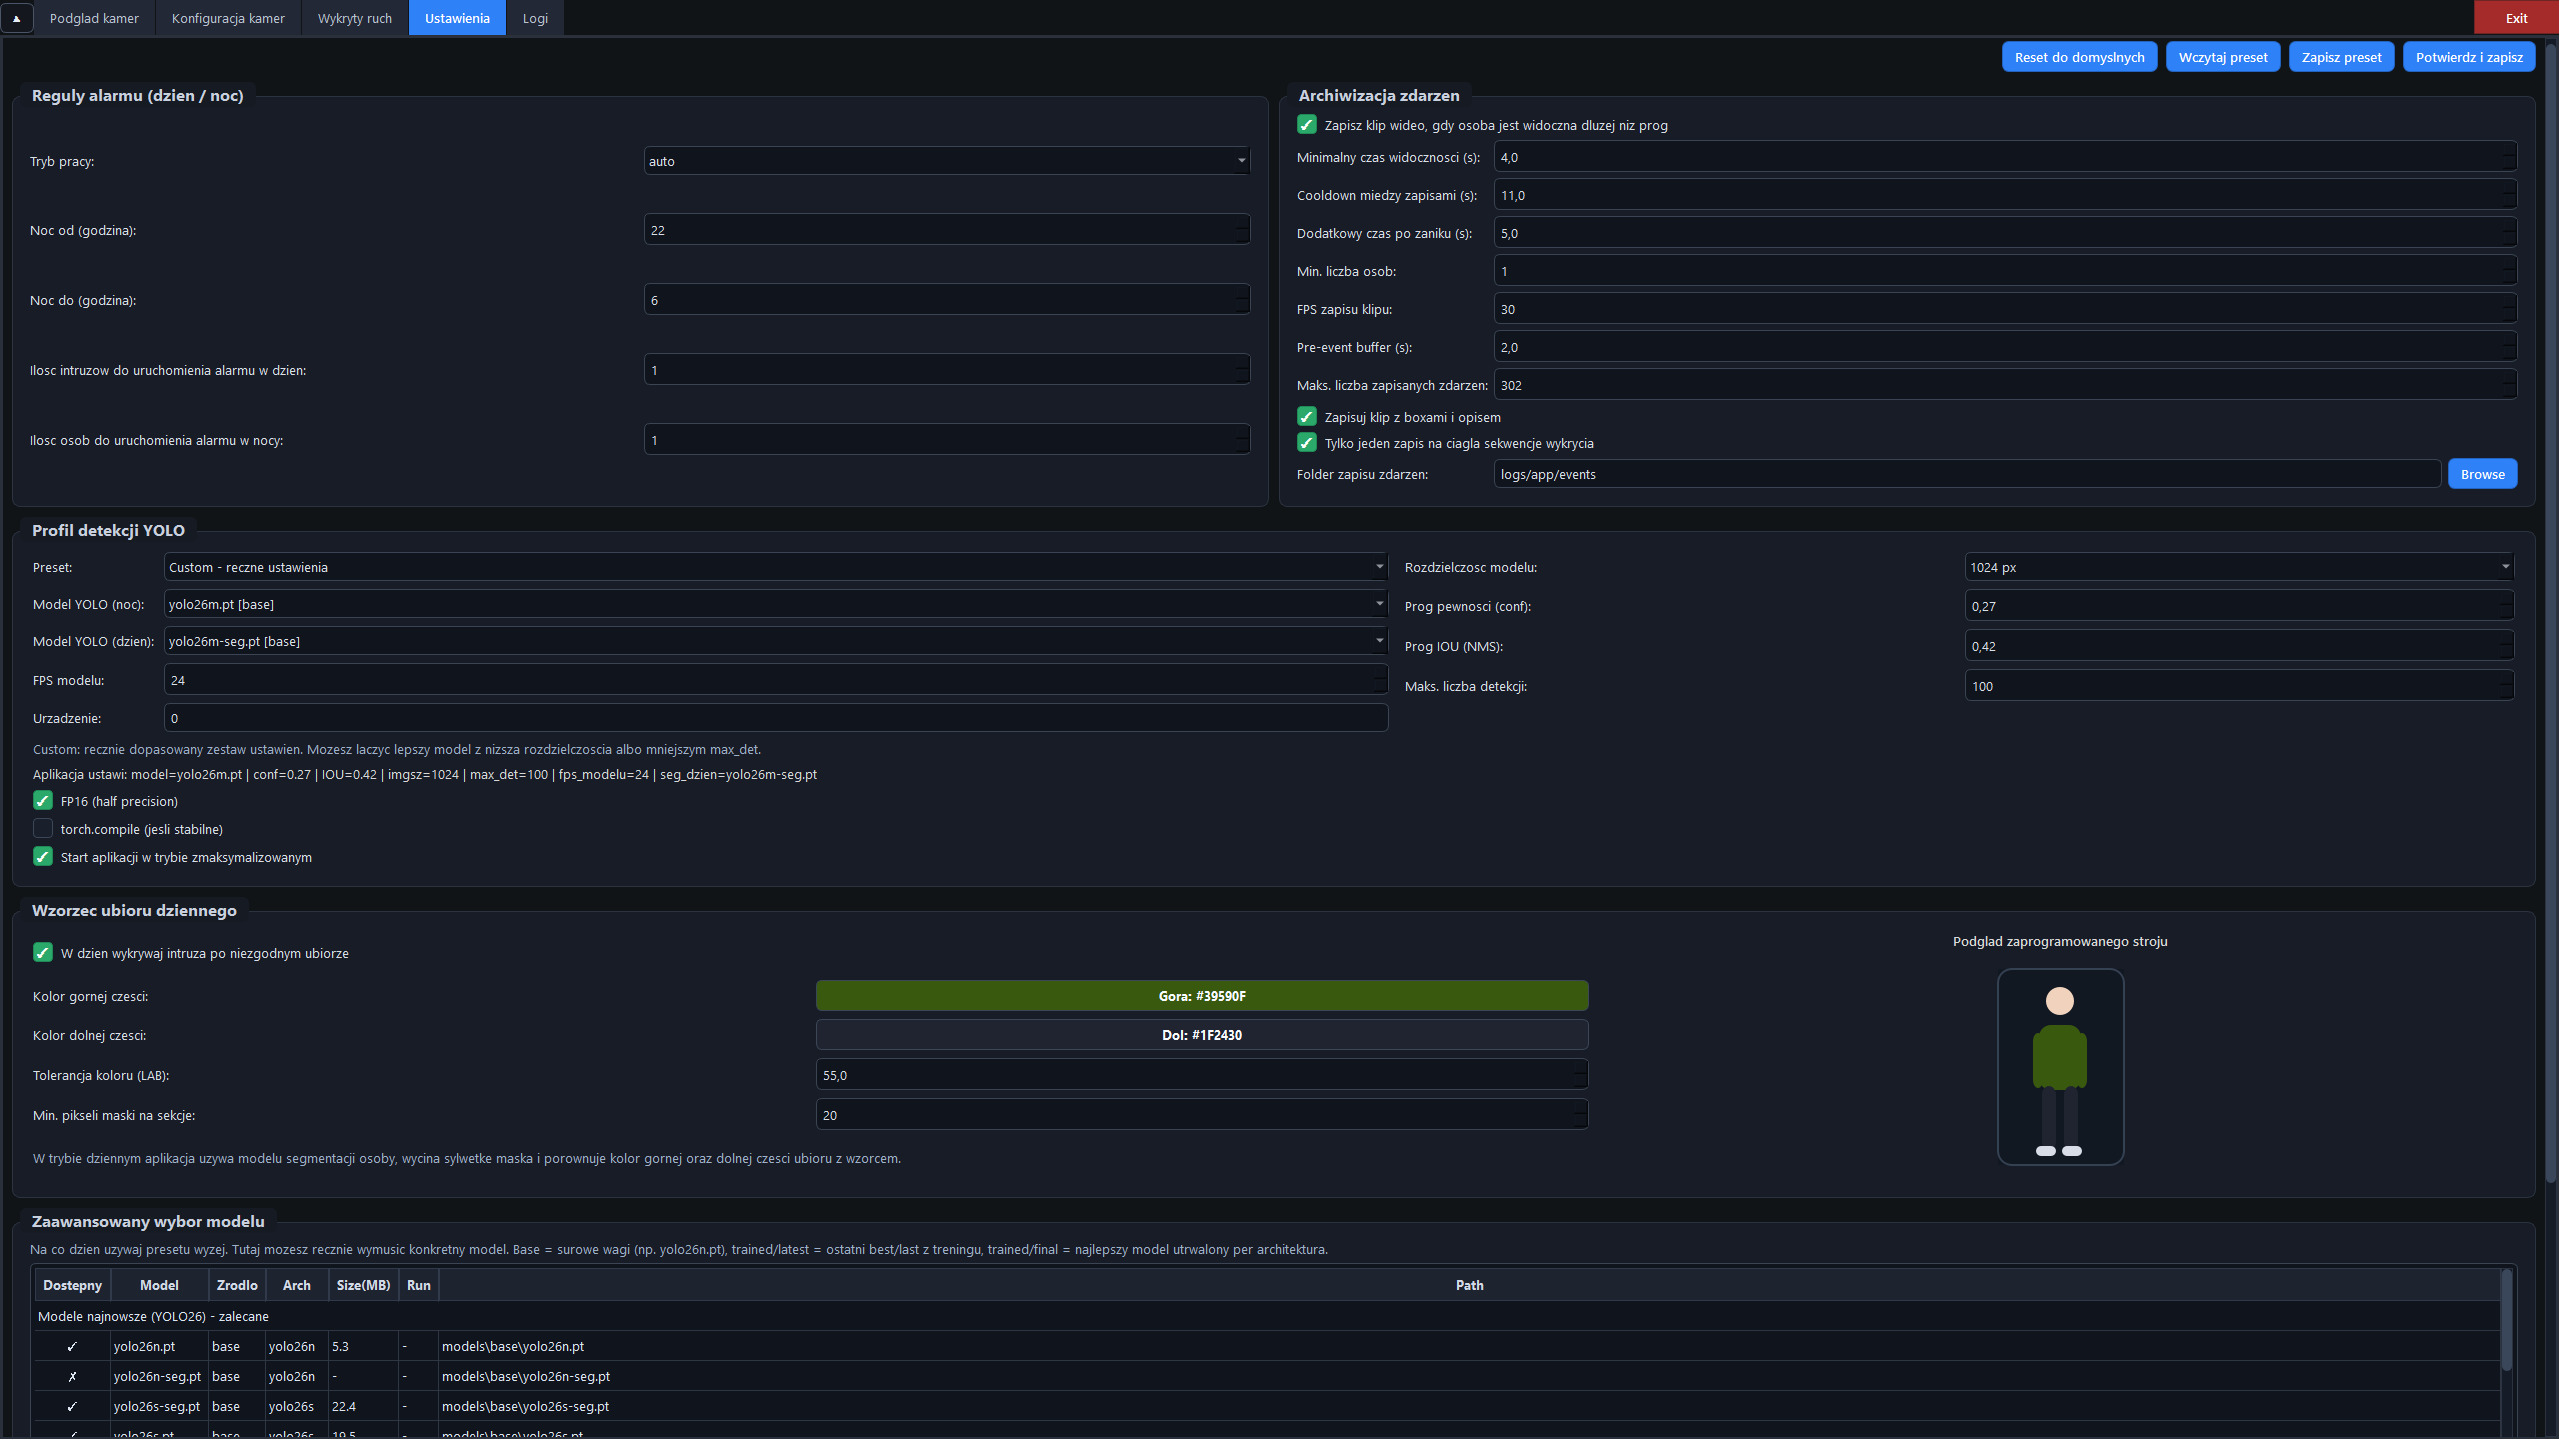
\includegraphics[width=0.95\textwidth]{rys/zakladka-ustawienia.png}
\caption{Panel ustawień aplikacji z konfiguracją reguł alarmu, modeli i wzorca ubioru.}
\label{fig:ustawienia}
\end{figure}
